%%%%%%%%%%%%%%%%%%%%%%%%%%%%%%%%%%%%%%%%%
% Beamer Presentation
% LaTeX Template
% Version 1.0 (10/11/12)
%
% This template has been downloaded from:
% http://www.LaTeXTemplates.com
%
% License:
% CC BY-NC-SA 3.0 (http://creativecommons.org/licenses/by-nc-sa/3.0/)
%
%%%%%%%%%%%%%%%%%%%%%%%%%%%%%%%%%%%%%%%%%

%----------------------------------------------------------------------------------------
%	PACKAGES AND THEMES
%----------------------------------------------------------------------------------------

\documentclass{beamer}

\mode<presentation> {

% The Beamer class comes with a number of default slide themes
% which change the colors and layouts of slides. Below this is a list
% of all the themes, uncomment each in turn to see what they look like.

%\usetheme{default}
%\usetheme{AnnArbor}
%\usetheme{Antibes}
%\usetheme{Bergen}
%\usetheme{Berkeley}
%\usetheme{Berlin}
%\usetheme{Boadilla}
%\usetheme{CambridgeUS}
%\usetheme{Copenhagen}
%\usetheme{Darmstadt}
%\usetheme{Dresden}
%\usetheme{Frankfurt}
%\usetheme{Goettingen}
%\usetheme{Hannover}
%\usetheme{Ilmenau}
%\usetheme{JuanLesPins}
%\usetheme{Luebeck}
\usetheme{Madrid}
%\usetheme{Malmoe}
%\usetheme{Marburg}
%\usetheme{Montpellier}
%\usetheme{PaloAlto}
%\usetheme{Pittsburgh}
%\usetheme{Rochester}
%\usetheme{Singapore}
%\usetheme{Szeged}
%\usetheme{Warsaw}

% As well as themes, the Beamer class has a number of color themes
% for any slide theme. Uncomment each of these in turn to see how it
% changes the colors of your current slide theme.

%\usecolortheme{albatross}
%\usecolortheme{beaver}
%\usecolortheme{beetle}
%\usecolortheme{crane}
%\usecolortheme{dolphin}
%\usecolortheme{dove}
%\usecolortheme{fly}
%\usecolortheme{lily}
%\usecolortheme{orchid}
%\usecolortheme{rose}
%\usecolortheme{seagull}
\usecolortheme{seahorse}
%\usecolortheme{whale}
%\usecolortheme{wolverine}

%\setbeamertemplate{footline} % To remove the footer line in all slides uncomment this line
%\setbeamertemplate{footline}[page number] % To replace the footer line in all slides with a simple slide count uncomment this line

%\setbeamertemplate{navigation symbols}{} % To remove the navigation symbols from the bottom of all slides uncomment this line
}

\usepackage{graphicx} % Allows including images
\usepackage{booktabs} % Allows the use of \toprule, \midrule and \bottomrule in tables
\usepackage[utf8]{inputenc}
\usepackage[spanish]{babel}
\decimalpoint
%\usecolortheme[rgb={0.6,0.3,0.2}]{structure} % para setear color
%----------------------------------------------------------------------------------------
%	TITLE PAGE
%----------------------------------------------------------------------------------------

\title[Propuesta de Tesis De Magíster]{Ensamble de Modelos Sintácticos y Semánticos para la Evaluación Automática de Ensayos} % The short title appears at the bottom of every slide, the full title is only on the title page

\author{Diego Palma S.} % Your name
\institute[UDEC] % Your institution as it will appear on the bottom of every slide, may be shorthand to save space
{
Profesor Supervisor: John Atkinson \\
\medskip
Universidad de Concepción \\ % Your institution for the title page
\medskip
\textit{dipalma@udec.cl} % Your email address
}
\date{\today} % Date, can be changed to a custom date

\begin{document}

\begin{frame}
\titlepage % Print the title page as the first slide
\end{frame}

\begin{frame}
\frametitle{Contenido} % Table of contents slide, comment this block out to remove it
\tableofcontents % Throughout your presentation, if you choose to use \section{} and \subsection{} commands, these will automatically be printed on this slide as an overview of your presentation
\end{frame}

%----------------------------------------------------------------------------------------
%	PRESENTATION SLIDES
%----------------------------------------------------------------------------------------

%------------------------------------------------
\section{Introducción} % Sections can be created in order to organize your presentation into discrete blocks, all sections and subsections are automatically printed in the table of contents as an overview of the talk
%------------------------------------------------

\begin{frame}
\frametitle{Introducción}
\begin{itemize}
\item En la actualidad, un tema bastante debatido es la capacidad de redacción y comprensión que debiesen tener las personas que egresan del sistema escolar.
\item Una mala redacción tiene consecuencias relevantes en la vida de una persona.
\item Un buen texto, debe cumplir con dos propiedades fundamentales: {\em coherencia} y {\em cohesión}.
\item Una forma de ayudar a los estudiantes a mejorar sus capacidades de escritura y expresión de ideas, es produciendo textos que sean corregidos por un experto que le entregue retroalimentación al estudiante.
\item Tener personal especializado disponible todo el tiempo es costoso.
\end{itemize}
\end{frame}

%------------------------------------------------

\begin{frame}
\frametitle{Introducción}
\begin{block}{Hipótesis}
Un método de evaluación de textos que considere características sintácticas y semánticas para evaluar coherencia textual será más efectivo para la tarea de evaluación automática de ensayos en comparación métodos que utilicen medidas superficiales estadísticas.
\end{block}

\end{frame}

\begin{frame}
\begin{block}{Objetivos}
\begin{itemize}
	\item Objetivo General
	\begin{itemize}
		\item Desarrollar un método computacional que permita evaluar automáticamente textos en forma de ensayos considerando aspectos de coherencia textual.
	\end{itemize}
	\item Objetivos Específicos
	\begin{itemize}
		\item Analizar estrategias de evaluación de ensayos en forma de texto, basados tanto en modelos de estadísticos, como en teoría de discurso.
		\item Desarrollar una estrategia que considere coherencia a nivel de contenido y sintaxis.
		\item Crear un prototipo para realizar las pruebas.
		\item Evaluar el modelo propuesto.
	\end{itemize}
\end{itemize}
\end{block}
\end{frame}
%------------------------------------------------

\section{Trabajo Relacionado}
\begin{frame}
\frametitle{Trabajo Relacionado}
Métodos basados en características superficiales:

\begin{itemize}
\item Representan los textos como un conjunto de características que se utilizan como medidas indirectas de propiedades del texto tales como: Coherencia, cohesión, contenido.
\item La nota se calcula como una suma ponderada de estas características (generalmente se utiliza regresión). El primer sistema exitoso (PEG) utilizaba regresión lineal.
\item Para obtener la ponderación de cada característica, se requiere tener un conjunto de ensayos previamente evaluados.
\begin{block}{Similaridad Contextual}
\begin{equation}
	Nota = \beta_0 + \sum_{i=1}^n \beta_i P_i
\end{equation}
\end{block}


\end{itemize}

\end{frame}

%------------------------------------------------

\begingroup
\small
\begin{frame}
\frametitle{Trabajo Relacionado}
Modelo de Espacio Vectorial

\begin{figure}
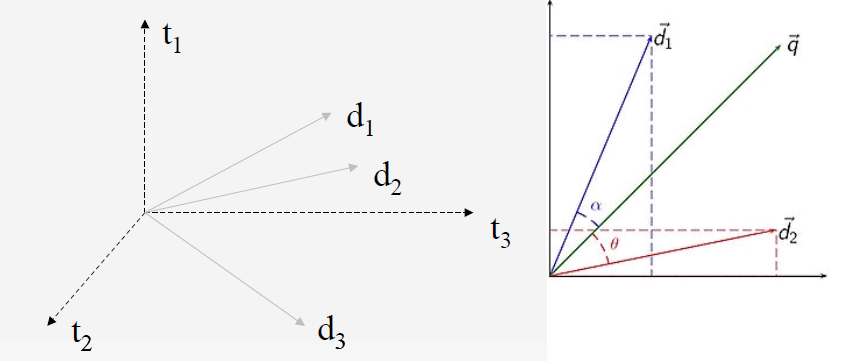
\includegraphics[width=0.4\linewidth]{fig1.png}
\end{figure}

\begin{itemize}
\item Se representan los documentos en un espacio vectorial con muchas dimensiones.
\item Se puede definir una medida de similitud entre documentos (por ejemplo coseno).
\item Método presenta algunos problemas.
\begin{block}{Similitud Coseno}
\begin{equation}
	cos(d_i, d_j) = \frac{d_i \cdot d_j}{\|d_i\| \|d_j\|}
\end{equation}
\end{block}

\end{itemize}

\end{frame}
\endgroup

%------------------------------------------------

\begin{frame}
\frametitle{Trabajo Relacionado}
Reducción Dimensional

Existen diversos problemas en utilizar un método de espacio vectorial, tales como:
\begin{itemize}
\item Polisemia (sim $<$ cos)
\item Sinónimos (sim $>$ cos)
\item Relaciones (ej: doctor/paciente/enfermera/tratamiento)
\item Matriz dispersa
\end{itemize}

\end{frame}

%------------------------------------------------

\begin{frame}
\frametitle{Trabajo Relacionado}
Análisis Semántico Latente (LSA)

\begin{itemize}
\item Utiliza una técnica de reducción dimensional conocida como descomposición de valores singulares.
\item El espacio dimensional reducido se le denomina espacio semántico.
\item Se identifican conceptos ocultos (latentes).
\item Se comparan los documentos en el espacio semántico obtenido.
\end{itemize}

\end{frame}

%------------------------------------------------

\begin{frame}
\frametitle{Trabajo Relacionado}

GLSA (Generalized Latent Semantic Analysis)
\begin{itemize}
\item Variación de LSA, que utiliza n-gramas en lugar de documentos.
\item Permite, por ejemplo, hacer distinción entre ``Literatura Fantástica'' con ``Fantástica Literatura''.
\item Considera orden de las palabras.
\item Sin embargo tiene algunas falencias: Alta dimensionalidad del espacio vectorial, alto grado de dispersión. La descomposición de valores singulares es costosa computacionalmente y crece con el orden de los n-gramas (explosión combinatoria).
\end{itemize}

\end{frame}

%------------------------------------------------

\begin{frame}
\frametitle{Trabajo Relacionado}

Probabilistic Latent Semantic Analysis
\begin{itemize}
\item Ni LSA ni GLSA logran solucionar el problema de la polisemia.
\item Otro problema relevante es que el espacio semántico obtenido es difícil de interpretar.
\item PLSA se fundamenta en un modelo probabilístico denominado {\em Aspect Model}, el cual expresa que las variables ocultas (tópicos) están asociadas a las variables observadas.

\begin{figure}
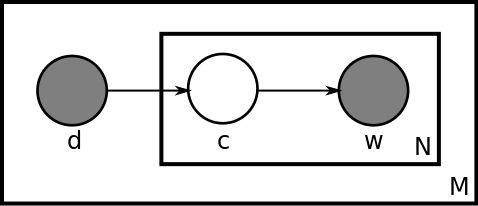
\includegraphics[width=0.5\linewidth]{../figure_plsa.png}
\end{figure}
\end{itemize}

\end{frame}

%------------------------------------------------

\begin{frame}
\frametitle{Trabajo Relacionado}

Algunas ventajas de PLSA:
\begin{itemize}
\item Modelo con base estadística sólida, con parámetros bien definidos que tienen una interpretación probabilística clara (variables latentes como tópicos).
\item Se puede utilizar teoría estadística para la selección del modelo (es decir, cantidad de dimensiones).
\item Logra solventar el problema de la polisemia.

\end{itemize}
\end{frame}

%------------------------------------------------

\begin{frame}
\frametitle{Trabajo Relacionado}

Métodos basados en teoría de discurso:
\begin{itemize}
\item Los métodos descritos hasta ahora, consideran los documentos como un conjunto de palabras independientes (modelo de bolsa de palabras).
\item El orden importa, pues afecta a la coherencia textual. La {\em teoría del centrado} establece que cada segmento de un texto (enunciados u oraciones) tiene asociado un centro (los cuales pueden ser pronombres, nombres, objetos, etc.).
\item La teoría define cuatro tipo de transiciones, las cuales sirven para evaluar qué tan coherente es un texto.
\end{itemize}

\begin{figure}
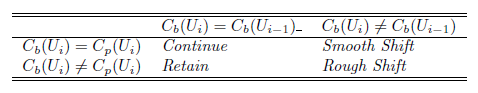
\includegraphics[width=0.5\linewidth]{fig2.png}
\end{figure}

\end{frame}

%------------------------------------------------

\begin{frame}
\frametitle{Trabajo Relacionado}
Ejemplo:
\begin{figure}
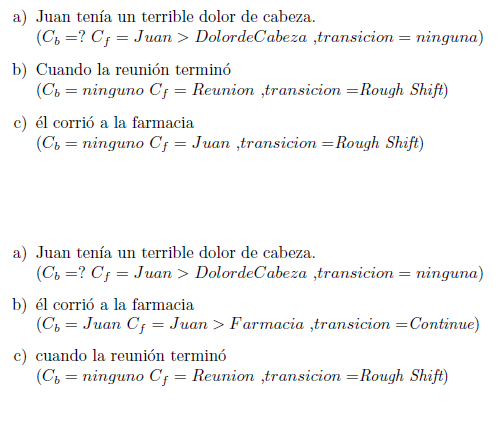
\includegraphics[width=0.5\linewidth]{fig3.png}
\end{figure}

\end{frame}

%------------------------------------------------

\begin{frame}
\frametitle{Trabajo Relacionado}

Método de evaluación de coherencia textual basado en teoría del centrado

\begin{itemize}
\item Se asume que existen ciertas transiciones que ocurren en textos coherentes.
\item La idea es, representar un texto como un conjunto de oraciones, donde cada entidad del texto tiene cambios de rol (transiciones) a lo largo de las oraciones. Estos cambios de rol, representan cómo van presentando las ideas del texto.
\end{itemize}

\end{frame}

%------------------------------------------------

\begin{frame}
\frametitle{Trabajo Relacionado}
Ejemplo de documento representado como una matriz de entidades.
\begin{figure}
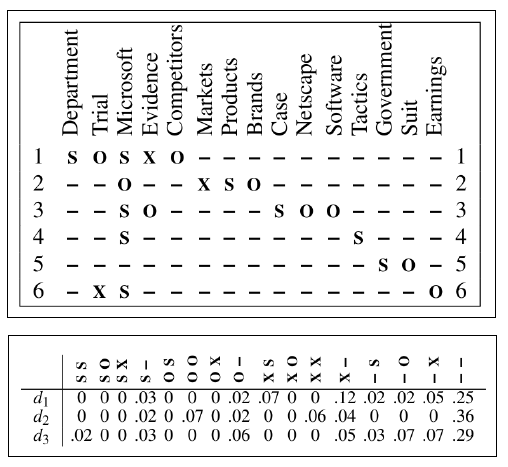
\includegraphics[width=0.5\linewidth]{fig4.png}
\end{figure}

\end{frame}

%----------------------------------------------------------------------------------------

\section{Propuesta}
\begin{frame}
\frametitle{Propuesta}
Se propone combinar los distintos métodos para obtener un método que considere distintos aspectos de la coherencia textual.

\begin{itemize}
\item Se propone utilizar medidas estadísticas que reflejan parcialmente características intrínsecas de los ensayos.
\item Utilizando un modelo de espacio vectorial se pueden evaluar algunos aspectos en relación a la semántica del texto.
\item Posteriormente, para considerar el orden de las ideas, se propone adaptar los métodos de evaluación de coherencia textual basados en teoría del discurso, para ser utilizados en el contexto de la evaluación automática de ensayos.
\item Finalmente, se propone combinar estos métodos.

\end{itemize}

\end{frame}

%-----------------------------------------------------------------------------------------
\section{Metodología}
\begin{frame}
\frametitle{Metodología}
\begin{enumerate}
	\item Revisión bibliográfica de métodos para evaluación de coherencia a nivel de discurso.
	
	\item Establecer una representación de textos con la que se pueda modelar la semántica del contenido textual.
	
	\item Recopilación de datos de ensayos evaluados por humanos, los cuales se limpiarán y prepararán para utilizarlos en el método a desarrollar.
	
	\item Desarrollo de un método de evaluación que considere sintaxis y semántica del ensayo a evaluar.
	
	\item Implementación de un prototipo computacional de los distintos métodos propuestos en la literatura, con la finalidad de realizar experimentos que validen la hipótesis.
	
	\end{enumerate}
\end{frame}

\begin{frame}
\frametitle{Metodología}
\begin{enumerate}
\setcounter{enumi}{5}
	\item Evaluación del método propuesto y comparación con otros métodos existentes en la literatura, para ello se utilizarán métricas tales como:
	
	\begin{itemize}
		\item {\em Exact Agreement}: Mide la proporción de ensayos que fueron calificados igualmente por el evaluador humano y el método computacional.
		\item {\em Adjacent Agreement}: Mide la proporción ensayos que fueron evaluados igual por el evaluador humano y el método computacional o que difieren en a lo más 1 punto (de calificación).
		\item {\em Quadratic Weighted Kappa}: Mide el grado de acuerdo entre los puntajes asignados por dos evaluadores. Su valor máximo es 1, si los evaluadores están completamente de acuerdo, si hay desacuerdo, la métrica puede tomar valores negativos.
		\item {\em Correlación de Spearman}: Mide qué tan buena es la relación entre la evaluación humana y la automática.
	\end{itemize}

\end{enumerate}

\end{frame}

%----------------------------------------------------------------------------------------
\section{Plan de Trabajo}
\begin{frame}
\frametitle{Plan de Trabajo}
\begin{itemize}
	\item Revisión bibliográfica de métodos de evaluación de coherencia textual, basados en teoría de discurso - Mes 1
	\item Diseño de un método automático para evaluar ensayos - Meses 2 - 3
	\item Implementación de métodos en el estado del arte, para posteriormente comparar con lo propuesto.
	\item Ensamble de modelos que consideren sintaxis y semántica - Mes 2
	\item Crear prototipo para realizar pruebas - Mes 3
	\item Evaluar rendimiento del modelo y comparar con modelos del estado del arte - Mes 4
\end{itemize}
\end{frame}

%----------------------------------------------------------------------------------------
\begin{frame}
\Huge{\centerline{FIN}}
\end{frame}

%----------------------------------------------------------------------------------------

\end{document} 